% Relatório final (KAN-10): CIN0144, Tema 8, Praso: Previsão de Inadimplência.
% Baseado no template IEEEtran (bare_conf.tex) da disciplina no Overleaf.
%
% Limite: 8 páginas. Entrega no Classroom até 02/12/2026; apresentação em 03/12.
%
% Para compilar no Overleaf:
%   1. envie este arquivo e as figuras usadas de reports/figures/ para a pasta figuras/ do projeto;
%   2. o IEEEtran.cls já vem instalado no Overleaf.
%
% Os textos em azul (\nota{...}) marcam o que ainda falta, com o roteiro e os
% números de cada parte. Substitua cada um pelo texto final e apague o \nota.

\documentclass[conference]{IEEEtran}

\usepackage[utf8]{inputenc}
\usepackage[T1]{fontenc}
\usepackage[brazilian]{babel}
\usepackage{graphicx}
\usepackage{booktabs}
\usepackage{amsmath}
\usepackage{xcolor}
\usepackage{url}
\usepackage{cite}

\graphicspath{{figuras/}{../reports/figures/}}

% Marca o que ainda falta. Sai do texto final.
\newcommand{\nota}[1]{\textcolor{blue}{[#1]}}

\begin{document}

\title{Previsão de Inadimplência de Varejistas da Praso\\com Modelos de Aplicação e Comportamental}

\author{
\IEEEauthorblockN{Luiz Miguel Freitas da Silva}
\IEEEauthorblockA{Centro de Informática - UFPE\\
Recife, Brasil\\
lmfs3@cin.ufpe.br}
\and
\IEEEauthorblockN{Mirella Laura Fontinelle Martins}
\IEEEauthorblockA{Centro de Informática - UFPE\\
Recife, Brasil\\
mlfm@cin.ufpe.br}
\and
\IEEEauthorblockN{Severino João da Cruz Júnior}
\IEEEauthorblockA{Centro de Informática - UFPE\\
Recife, Brasil\\
sjcj2@cin.ufpe.br}
\and
\IEEEauthorblockN{Willian Neves Rupert Jones}
\IEEEauthorblockA{Centro de Informática - UFPE\\
Recife, Brasil\\
wnrj@cin.ufpe.br}
}

\maketitle

\begin{abstract}
A Praso vende a prazo para pequenos varejistas e precisa estimar o risco de inadimplência de cada cliente. Com dados reais de 3.000 clientes do Ceará, dos quais 31,3\% ficaram inadimplentes, construímos dois modelos: um de aplicação, que usa apenas o cadastro e serve para clientes novos, e um comportamental, que acrescenta o histórico de pedidos disponível para 22\% da base. A análise exploratória mostrou que o risco vem da combinação de três fontes (maturidade da empresa, histórico na Serasa e tipo de negócio), o que motivou modelos de árvore. O modelo de aplicação, um XGBoost calibrado com 10 variáveis escolhidas por ablação, obteve ROC-AUC de 0,777 na validação cruzada e 0,798 no conjunto de teste. O modelo comportamental, uma Random Forest treinada nos 664 clientes com pedidos, eleva o AUC nesses clientes de 0,691 para 0,766 na validação, com o atraso nos pagamentos como principal sinal. \nota{Uma frase sobre a política de crédito (KAN-9).} A principal limitação é a ausência de datas na base, que impede garantir que as variáveis sejam anteriores à inadimplência.
\end{abstract}

\begin{IEEEkeywords}
risco de crédito, inadimplência, gradient boosting, ROC-AUC
\end{IEEEkeywords}

% =====================================================================
\section{Introdução}

A Praso fornece mercadorias a pequenos varejistas com pagamento a prazo. Vender a prazo amplia o acesso desses clientes a crédito, mas expõe a empresa ao risco de não receber. Decidir a quem conceder crédito, e com qual limite, exige estimar a probabilidade de inadimplência de cada cliente.

O problema tem dois momentos. No cadastro, a empresa conhece apenas dados da empresa cliente (idade do CNPJ, capital social, atividade econômica), consultas a birôs de crédito e presença em plataformas digitais. Depois que o cliente começa a comprar, o histórico de pedidos (valores e atrasos) passa a informar também. Por isso, este trabalho constrói dois modelos, como pedido pela Praso:
\begin{itemize}
\item \textbf{modelo de aplicação}, só com dados do cadastro, para avaliar clientes novos;
\item \textbf{modelo comportamental}, que acrescenta o histórico de pedidos.
\end{itemize}

A métrica principal é o ROC-AUC, que mede a capacidade de ordenar os clientes por risco. As principais contribuições são: (i) uma análise exploratória orientada por hipóteses, que identifica as fontes de risco e suas interações; (ii) um modelo de aplicação com seleção de variáveis por ablação e comparação estatística entre algoritmos; (iii) a medida do ganho do histórico de pedidos sobre o cadastro; e (iv) uma discussão de como usar os scores numa política de crédito.

% =====================================================================
\section{Análise de Dados e Feature Engineering}

\subsection{Análise Exploratória dos Dados}

\subsubsection{Análise Exploratória Estrutural}
A base tem duas tabelas fornecidas pela Praso sob termo de confidencialidade, por isso apresentamos apenas agregados. A tabela de clientes tem 3.000 linhas e 19 colunas, uma por cliente, todos do Ceará (36 municípios). O alvo é binário: 940 clientes (31,3\%) ficaram inadimplentes, um desbalanceamento moderado. A tabela de pedidos tem 1.977 pedidos de 664 clientes (22\% da base), entregues entre abril de 2022 e abril de 2026, 77\% deles em 2023. Muitas variáveis vêm em faixas, inclusive o capital social, a idade do CNPJ e o valor e o atraso dos pedidos. Não há linhas nem chaves duplicadas, nem valores fora do formato esperado.

Dois pontos estruturais limitam o trabalho. Primeiro, a base não tem nenhuma data de cadastro nem de observação da inadimplência. Segundo, cada cliente tem no máximo 3 pedidos, o que sugere um recorte do histórico, e não o histórico completo.

\subsubsection{Análise de Valores Faltantes e Outliers}
A lista de credores da Serasa é nula em 82\% dos clientes, o que em geral significa ``sem credores''. Porém, 97 clientes têm negativação e nenhum credor listado, e para eles o nulo pode ser informação faltando. A nota do Google Maps existe para só 34 clientes, e a indicação de website é nula exatamente para quem não está no Maps, o que a torna uma cópia da presença na plataforma. Negativações e protestos têm cauda longa (máximos de 141 e 79), mas os valores altos são plausíveis.

\subsubsection{Análise Univariada}
A idade do CNPJ é a variável mais forte: a taxa de inadimplência cai de 57\% nas empresas mais novas para 6\% nas mais antigas, com degraus por volta de 1.600 e 5.000 dias. Mesmo assim, sozinha ela tem ROC-AUC de apenas 0,639. Na Serasa, o número de credores leva a taxa de 28\% a 72\%, e ter o sócio negativado, de 22\% para 42\%. Empresário individual inadimple mais que LTDA (34,7\% contra 21,3\%), e há segmentos com taxas de 19\% a 44\%. A presença no iFood ou no Google Maps e os protestos quase não informam.

\subsubsection{Análise Bivariada}
A correlação de Spearman mostra que o número de credores e o de negativações medem quase a mesma coisa ($\rho = 0{,}90$). Entre as categóricas, o V de Cramér indica que os três níveis do CNAE são redundantes entre si (0,89 a 0,94), enquanto o segmento da Praso não é um recorte do CNAE (V = 0,58) e se associa mais ao alvo.

\subsubsection{Análise Multivariada}
Os sinais interagem. Ter dois ou mais credores anula a proteção da idade: uma empresa com mais de 14 anos nessa situação inadimple 41,7\%, contra 5,6\% sem credores (Fig.~\ref{fig:interacao}). O sócio negativado quase não muda o risco de empresas com menos de um ano, que já é alto, mas dobra a taxa entre 1 e 14 anos. Combinando só duas variáveis, a taxa vai de 3,8\% a 85,7\%. Algumas diferenças diretas também enganam: ajustadas pela idade, as fontes de aquisição 2 e 5 ficam igualmente arriscadas (cerca de 41\%). Essas interações motivaram o uso de modelos de árvore.

\begin{figure}[htbp]
\centering
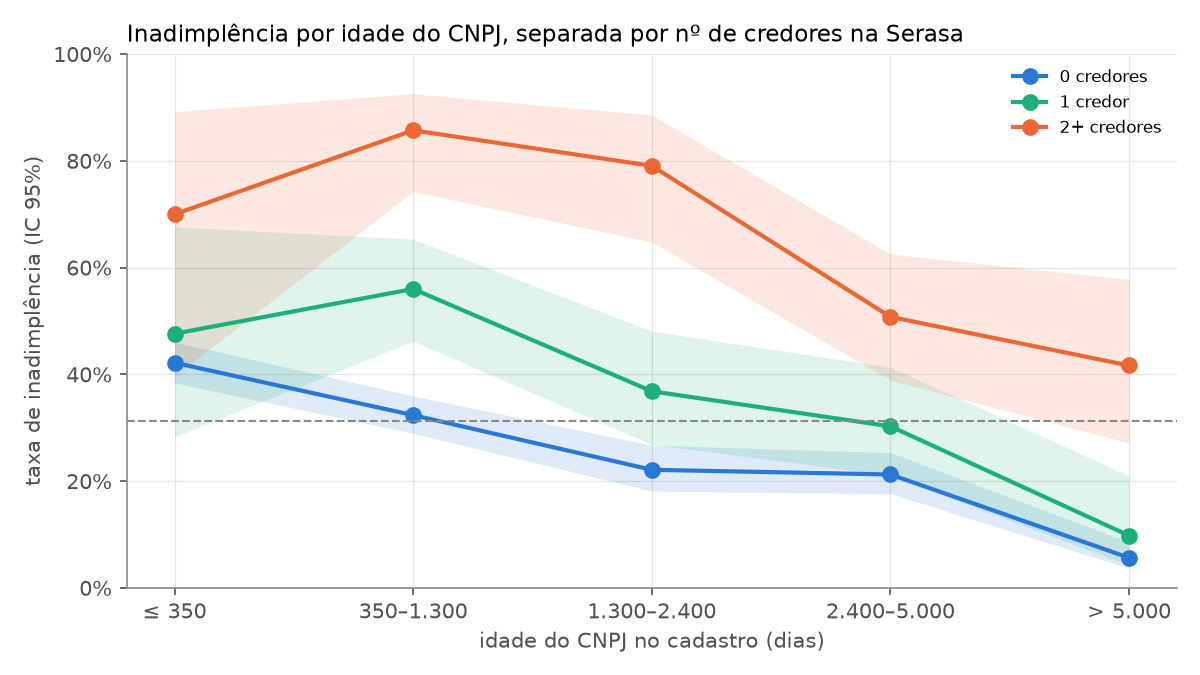
\includegraphics[width=\columnwidth]{eda_interacao_idade_credores}
\caption{Taxa de inadimplência por idade do CNPJ e número de credores na Serasa.}
\label{fig:interacao}
\end{figure}

\subsection{Pré-processamento dos Dados}

A limpeza compartilhada entre os dois modelos só faz o que não perde informação: converte tipos e datas, ordena os pedidos e transforma as faixas em categóricas ordenadas pelo limite inferior. Nenhum registro é removido.

\subsubsection{Tratamento de Valores Faltantes}
Em vez de imputar, os nulos com significado viram variáveis. Os negativados sem credor listado recebem a flag \texttt{negativado\_sem\_credor}, e a ausência nas plataformas vira ``sem contagem''. Nos dois pedidos com valor ou atraso nulo, o nulo é ignorado só na estatística da coluna que falta.

\subsubsection{Tratamento de Outliers}
As contagens altas da Serasa foram mantidas: são plausíveis, e os modelos de árvore usam só a ordem dos valores, então a cauda longa não distorce o ajuste.

\subsubsection{Detecção e Tratamento de Duplicadas}
Não há linhas nem chaves duplicadas. Os 74 pares de pedidos do mesmo cliente no mesmo dia foram mantidos como pedidos distintos.

\subsubsection{Feature Scaling}
Os modelos finais são de árvore e dispensam normalização. Na regressão logística, usada como comparação, as variáveis numéricas são padronizadas.

\subsubsection{Encoding de Variáveis Categóricas}
As faixas viram a posição da faixa (codificação ordinal). Nas categóricas, as categorias com menos de 30 clientes no treino formam um grupo só; para as árvores, cada categoria vira um código, e para a regressão logística, uma coluna \textit{one-hot}. O \textit{target encoding} da classe do CNAE foi testado e não superou o agrupamento das raras. Toda transformação que aprende dos dados fica dentro do \texttt{Pipeline} do scikit-learn e é ajustada só no treino.

\subsection{Divisão dos Dados}
Sem datas, a divisão não pode ser temporal. Usamos uma divisão aleatória de 80/20, estratificada pelo alvo e pela presença de pedidos (semente 42): 2.400 clientes no treino e 600 no teste, ambos com 31,3\% de inadimplência e 22\% com pedidos. A estratificação pela presença de pedidos garante que os dois modelos sejam comparados nos mesmos clientes. No treino, todas as escolhas usam validação cruzada estratificada com 5 folds e 5 repetições. Como os folds repetidos reaproveitam clientes, as comparações pareadas usam o erro padrão corrigido de Nadeau e Bengio~\cite{nadeau2003}. O teste é usado uma única vez, na avaliação final.

\subsection{Feature Engineering}

\subsubsection{Modelo de aplicação}
A partir do cadastro, criamos 23 variáveis calculadas linha a linha, sem olhar o alvo: por exemplo, a posição da faixa de idade, o número de credores, flags por tipo de credor e a região do município. Para escolher as finais, fizemos uma ablação no treino com uma Random Forest de parâmetros fixos. Cada item é retirado e o ganho de AUC é medido nos mesmos folds; o item fica se o ganho passar de um erro padrão corrigido. A Fig.~\ref{fig:ablacao} mostra o resultado por bloco, partindo da idade sozinha (AUC 0,631). Nessa ordem, a Serasa acrescenta 0,100 e o tipo de negócio, 0,032; o bloco da empresa (capital social e natureza jurídica) quase nada acrescenta logo após a idade, mas acrescenta 0,009 quando retirado do modelo final, e por isso fica. Plataformas, negativações (redundantes com os credores), tipo de credor e divisão do CNAE saíram sem perda. O modelo final tem 10 variáveis: idade do CNPJ, capital social, natureza jurídica, número de credores, sócio negativado, negativado sem credor, fonte de aquisição, segmento, classe do CNAE e região, com AUC de 0,772, contra 0,765 com as 23.

Como não se sabe quando a Serasa foi consultada, medimos também a dependência desse bloco. Sem a Serasa, o AUC cai para 0,699, ainda bem acima da idade sozinha, e nos clientes sem nenhum registro na Serasa o modelo ordena quase tão bem quanto no total (0,767 contra 0,771).

\begin{figure}[htbp]
\centering
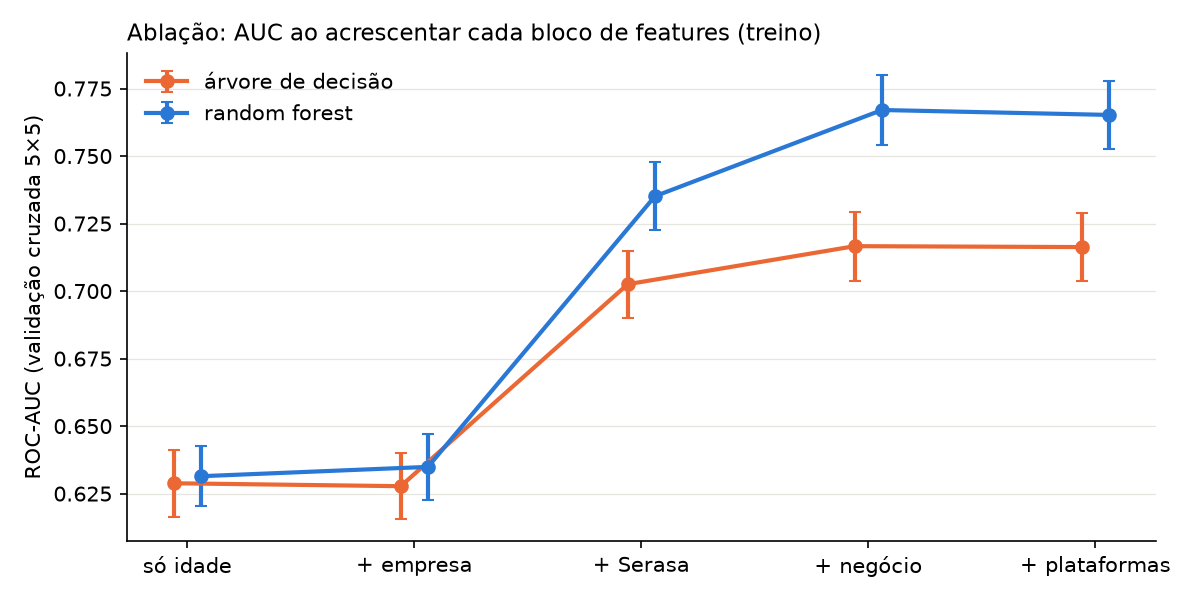
\includegraphics[width=\columnwidth]{kan5_ablacao}
\caption{Ablação das variáveis do modelo de aplicação: AUC na validação cruzada ao acrescentar cada bloco.}
\label{fig:ablacao}
\end{figure}

\subsubsection{Modelo comportamental}
Para cada cliente com pedidos, agregamos 16 variáveis sobre valor (mínimo, média, máximo), atraso (média, máximo, proporção de pedidos com atraso, atraso do último pedido, tendência) e ritmo de compra. As faixas viram o ponto médio. O número de pedidos não entra, porque quase todos os clientes têm 3, e não há recência absoluta, porque sem data de referência ela mediria a época, e não o comportamento.

Sem data, há duas hipóteses: (a) o último pedido é anterior à inadimplência e todos os pedidos entram; (b) o último pedido é o próprio evento e deve sair. Testamos as duas no histórico dos inadimplentes, com regra fixada antes de ver o resultado. Se (b) valesse, os inadimplentes com o último pedido em dia só seriam explicados por um histórico anterior de atrasos graves. Porém, 52 dos 110 inadimplentes do treino com pedidos têm o último pedido com até 2 dias de atraso, e nenhum dos 51 com histórico anterior atrasou mais de 15 dias antes dele. Seguimos a hipótese (a).

O sinal está no atraso (Fig.~\ref{fig:atraso}): quem atrasou mais de 2 dias inadimple mais, em qualquer posição do histórico, e a diferença é maior no pedido mais recente.

\begin{figure}[htbp]
\centering
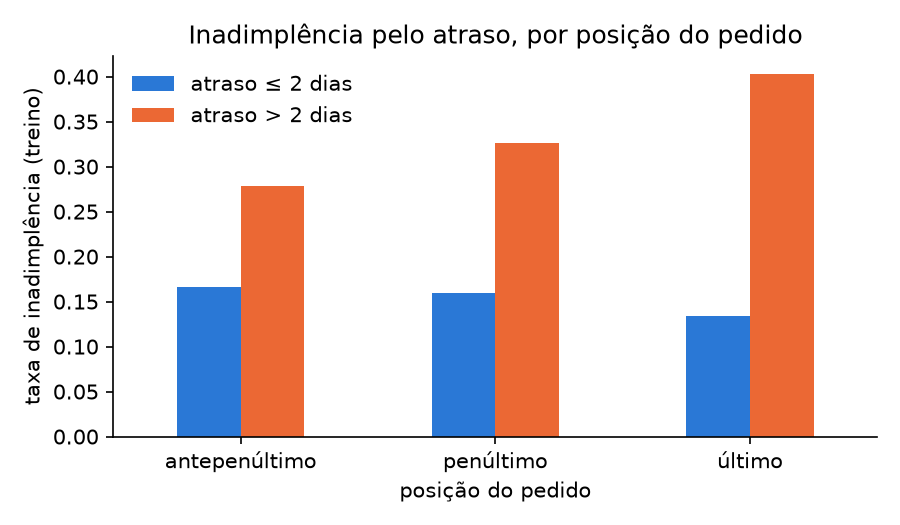
\includegraphics[width=\columnwidth]{kan7_atraso_por_posicao}
\caption{Taxa de inadimplência no treino com atraso de até 2 dias ou acima disso, por posição do pedido no histórico.}
\label{fig:atraso}
\end{figure}

% =====================================================================
\section{Modelagem}

Como o risco vem da combinação das variáveis e de degraus na idade (Seção II-A5), o modelo de aplicação usa principalmente modelos de árvore, que encontram essas interações sozinhos. Para cada modelo, uma busca aleatória sorteia configurações de um espaço de hiperparâmetros e mede cada uma nos 25 folds. Os espaços favorecem modelos regularizados, porque com 2.400 clientes árvores profundas e folhas pequenas decoram o treino. Como escolher a melhor entre muitas configurações tende a premiar a sorte, a escolha foi conferida separando as repetições: escolhendo só pelas repetições 1 e 2, a configuração vencedora de cada modelo é a mesma, e o ganho se mantém nas repetições 3 a 5.

\subsection{Linhas de Base: Árvore de Decisão e Regressão Logística}
\subsubsection{Conceitos Básicos}
A árvore de decisão divide os clientes recursivamente pela variável e pelo corte que mais separam o alvo. A regressão logística modela o log da razão de chances como uma combinação linear das variáveis.
\subsubsection{Justificativa}
São modelos interpretáveis, que servem de referência. A logística é a alternativa usual em crédito, e seus coeficientes repetem a análise exploratória: idade, credores e sócio negativado pesam mais.
\subsubsection{Espaço de Busca}
A árvore usa parâmetros fixos. Na logística, com regularização L2, a força $C$ é escolhida numa grade de 0,01 a 3, em que o AUC varia só de 0,758 a 0,762. Também testamos as interações da análise exploratória (idade $\times$ sócio e idade $\times$ credores), que não acrescentaram nada.
\subsubsection{Hiperparâmetros Selecionados}
Árvore com profundidade máxima 4 e pelo menos 30 clientes por folha; logística com $C = 0{,}03$.

\subsection{Random Forest}
\subsubsection{Conceitos Básicos}
A Random Forest~\cite{breiman2001} treina muitas árvores em amostras \textit{bootstrap} dos clientes, sorteando um subconjunto de variáveis em cada divisão, e faz a média das previsões.
\subsubsection{Justificativa}
É um \textit{ensemble} estável e pouco sensível aos hiperparâmetros, por isso foi usada na ablação, com 300 árvores e pelo menos 20 clientes por folha.
\subsubsection{Espaço de Busca}
Número mínimo de clientes por folha, número de variáveis por divisão e profundidade máxima (20 configurações).
\subsubsection{Hiperparâmetros Selecionados}
As melhores configurações usam folhas de 5 a 10 clientes com profundidade limitada (6 ou 10).

\subsection{Gradient Boosting: XGBoost e LightGBM}
\subsubsection{Conceitos Básicos}
O \textit{gradient boosting} ajusta árvores em sequência, cada uma corrigindo o erro das anteriores na direção do gradiente da perda. O XGBoost~\cite{chen2016} acrescenta regularização explícita; o LightGBM cresce as árvores por folha.
\subsubsection{Justificativa}
É a família com melhor desempenho típico em dados tabulares, e a regularização controla o \textit{overfitting} numa base pequena.
\subsubsection{Espaço de Busca}
Número de árvores, taxa de aprendizado, profundidade (ou número de folhas no LightGBM), peso ou número mínimo de clientes por folha, subamostragem de clientes e de variáveis e regularização L2, com 40 configurações por modelo.
\subsubsection{Hiperparâmetros Selecionados}
O modelo final é o XGBoost com 500 árvores, profundidade 5, taxa de aprendizado 0,01, 80\% dos clientes e 60\% das variáveis por árvore e regularização L2 = 10, seguido de calibração sigmoide para que o score seja uma probabilidade.

\subsection{Modelo Comportamental}
O modelo comportamental é treinado e avaliado só nos 664 clientes com histórico de pedidos (531 no treino, com 110 inadimplentes, e 133 no teste), com o mesmo split e os mesmos folds do modelo de aplicação, para que a comparação seja pareada. Quem não tem pedidos continua com o modelo de aplicação. O enunciado define o cliente ativo como quem comprou nos últimos 30 dias, mas sem data de referência esse corte não pode ser aplicado: a partir da data mais recente da base, sobraria um único cliente. Treinar com todos os clientes, com as variáveis de pedidos nulas para quem não tem histórico, daria AUC um pouco maior nas árvores (0,020 na Random Forest), mas misturaria duas populações com taxas diferentes (34\% e 21\%) e subestimaria o risco dos clientes com pedidos.

As variáveis são as 10 do modelo de aplicação, 6 de atraso (média, mediana, máximo, proporção de pedidos com atraso e com mais de 2 dias, e tendência) e o intervalo médio entre pedidos. Os blocos de pedidos entraram um de cada vez, com a mesma regra de um erro padrão. O atraso eleva o AUC de 0,691 para 0,754; o intervalo acrescenta 0,012, no limite da regra; o valor e o número de dias com pedido não acrescentam.

Os candidatos foram a regressão logística, com a mesma grade de $C$, e a Random Forest, o XGBoost e o LightGBM, com busca aleatória nos mesmos espaços do modelo de aplicação (20 configurações cada). Pela regra, fica o candidato mais simples que o melhor não supera por mais de um erro padrão: a Random Forest com os parâmetros da ablação (300 árvores, pelo menos 20 clientes por folha e raiz quadrada do número de variáveis por divisão). Treinada só nos clientes com pedidos, ela já sai calibrada (score médio de 20,7\% para 20,7\% observados), e a calibração sigmoide não reduz o erro de Brier, por isso não é usada.

% =====================================================================
\section{Análise e Comparação de Resultados}

A métrica principal é o ROC-AUC: a probabilidade de um inadimplente sorteado ter score maior que um adimplente sorteado. Ela não depende do corte nem é afetada pelo desbalanceamento, e corresponde ao uso do score para ordenar clientes. Na validação cruzada, os modelos são comparados nos mesmos folds, com o erro padrão corrigido; no teste, os intervalos de confiança vêm de \textit{bootstrap}. A calibração é avaliada à parte.

\begin{table}[htbp]
\caption{Modelo de aplicação: AUC na validação cruzada 5$\times$5}
\label{tab:aplicacao}
\centering
\begin{tabular}{lcc}
\toprule
Modelo & AUC val. & treino $-$ val. \\
\midrule
Só idade (Random Forest) & 0,631 & 0,024 \\
Árvore de decisão & 0,723 & 0,025 \\
Regressão logística & 0,762 & 0,011 \\
Random Forest sem tuning & 0,772 & 0,056 \\
Random Forest (busca) & 0,773 & 0,058 \\
LightGBM (busca) & 0,776 & 0,077 \\
\textbf{XGBoost (busca), final} & \textbf{0,777} & 0,070 \\
\bottomrule
\end{tabular}
\end{table}

A Tabela~\ref{tab:aplicacao} resume a comparação. A árvore de decisão (0,723) e a logística (0,762) ficam abaixo da Random Forest sem tuning. Os três modelos de árvore com busca chegam ao mesmo teto, perto de 0,776, o que indica que o limite está nos dados, e não no algoritmo. O XGBoost é o único que supera a Random Forest por mais de um erro padrão corrigido: o ganho é pequeno (+0,004), mas consistente, já que ele vence em 19 dos 25 folds. Os modelos que validam melhor também se ajustam mais ao treino (diferença de 0,070 no XGBoost), mas, na busca, tanto as configurações que decoram mais quanto as que decoram menos validam pior.

No teste, usado uma única vez, o modelo final obteve AUC de 0,798 (IC de 95\%: 0,757 a 0,835), contra 0,659 da idade sozinha e 0,746 da árvore de decisão (Fig.~\ref{fig:roc}). Entre o XGBoost, a Random Forest e a logística, o teste não separa: as diferenças são de até 0,006, com intervalos que cruzam o zero.

\begin{figure}[htbp]
\centering
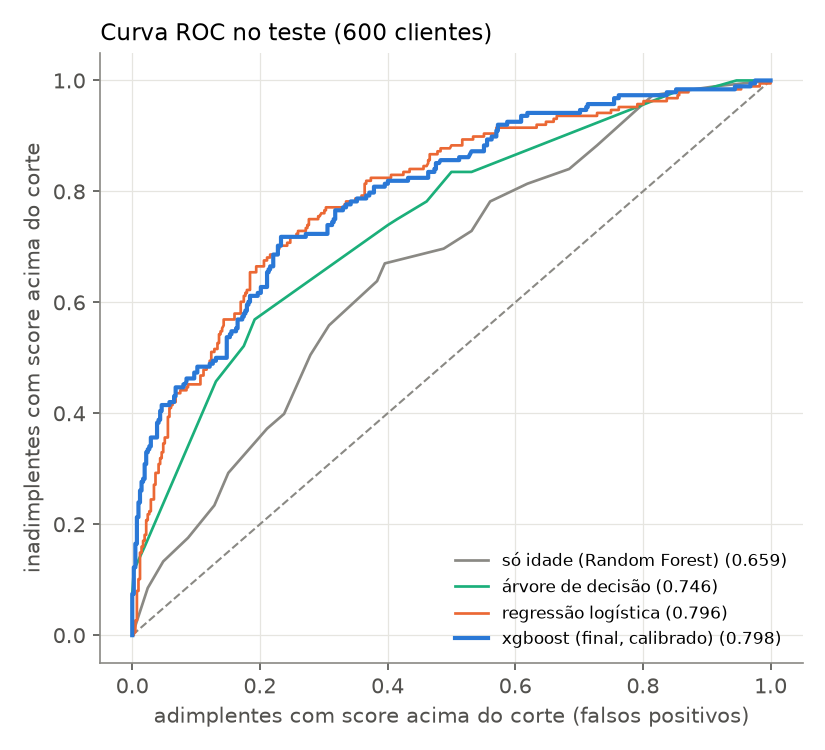
\includegraphics[width=0.85\columnwidth]{kan6_roc_teste}
\caption{Curvas ROC no conjunto de teste.}
\label{fig:roc}
\end{figure}

O score calibrado acompanha a taxa observada: a média é de 31,5\% no treino (fora da amostra) e 30,7\% no teste, para 31,3\% observados, e por decil de score a taxa vai de 5,0\% a 70,4\%. Nos clientes com histórico de pedidos, porém, o score superestima o risco (28,3\% contra 20,7\% observados), porque o modelo de aplicação não sabe quem tem histórico e esses clientes inadimplem menos.

Nos clientes com pedidos, o modelo comportamental eleva o AUC de validação de 0,691, o do modelo de aplicação nos mesmos clientes e folds, para 0,766 (+0,075, 2,0 erros padrão; Fig.~\ref{fig:comportamental}). Os modelos de árvore empatam entre si (0,766 a 0,772), e a logística fica em 0,748. No teste, o AUC é 0,740 (IC de 95\%: 0,638 a 0,835), contra 0,670 do modelo de aplicação nos mesmos 133 clientes. A diferença, de +0,070, vai na mesma direção da validação, mas o intervalo dela ($-0{,}060$ a $+0{,}203$) cruza o zero: com só 28 inadimplentes, o teste sozinho não confirma o ganho. A logística foi melhor no teste (0,789), mas os intervalos se sobrepõem quase inteiros, e escolher pelo teste seria usá-lo duas vezes. O score acompanha a taxa observada (22,0\% previsto para 21,1\% no teste) e, por decil, a inadimplência vai de 0\% a 60,4\% no treino.

\begin{figure}[htbp]
\centering
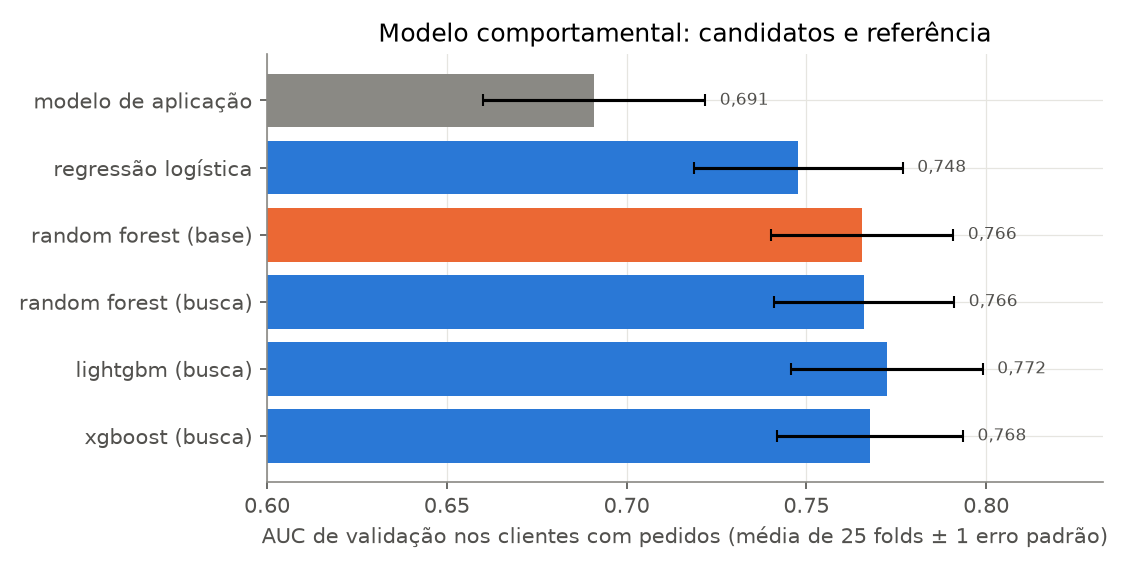
\includegraphics[width=\columnwidth]{kan8_comparacao}
\caption{Modelo comportamental: AUC de validação nos clientes com pedidos, com $\pm$1 erro padrão. Em destaque, o modelo escolhido; em cinza, o modelo de aplicação nos mesmos clientes.}
\label{fig:comportamental}
\end{figure}

% =====================================================================
\section{Conclusão e Discussão}

\nota{KAN-9: como usar os scores numa política de crédito (cortes pelos scores fora da amostra do treino, conferidos no teste; limite de crédito por faixa de risco; papel do componente comportamental).}

O risco de inadimplência dos clientes da Praso vem de três fontes: a maturidade da empresa, o histórico na Serasa e o tipo de negócio. Nenhuma variável resolve sozinha, mas a combinação delas leva o AUC de 0,639 (idade do CNPJ) para 0,777 na validação e 0,798 no teste. Com 2.400 clientes e 10 variáveis fortes, a escolha do algoritmo importa pouco: os modelos de árvore ordenam os clientes quase igual, e a regressão logística fica perto deles, como alternativa interpretável. No histórico de pedidos, o sinal está no atraso: nos clientes com pedidos, o modelo comportamental eleva o AUC de 0,691 para 0,766 na validação.

As principais limitações vêm dos dados. Sem nenhuma data, não é possível garantir que a consulta à Serasa e os pedidos sejam anteriores à inadimplência; o teste das hipóteses sobre o último pedido reduz, mas não elimina, esse risco. O histórico tem no máximo os 3 pedidos mais recentes de cada cliente, o que impede contar os pedidos e aplicar a definição de cliente ativo do enunciado. Só 28 inadimplentes do teste têm pedidos, o que deixa a avaliação do modelo comportamental com intervalos largos, e a escolha entre a logística e as árvores nesse modelo é decidida por margens pequenas. Também não está claro o que significa inadimplência para os 78\% de clientes sem nenhum pedido. Como trabalhos futuros, sugerimos obter as datas de cadastro e de observação do alvo, o que permitiria uma validação temporal, e um histórico de pedidos mais longo.

% =====================================================================
\begin{thebibliography}{1}

\bibitem{nadeau2003}
C.~Nadeau and Y.~Bengio, ``Inference for the generalization error,'' \emph{Machine Learning}, vol.~52, no.~3, pp. 239--281, 2003.

\bibitem{chen2016}
T.~Chen and C.~Guestrin, ``XGBoost: A scalable tree boosting system,'' in \emph{Proc. 22nd ACM SIGKDD}, 2016, pp. 785--794.

\bibitem{breiman2001}
L.~Breiman, ``Random forests,'' \emph{Machine Learning}, vol.~45, no.~1, pp. 5--32, 2001.

\end{thebibliography}

\end{document}
